\section{Overview}
\hspace{0.5cm} This chapter discusses the use the generalized range equation for jet aircraft and the simplifications known as the Br\'eguet range and endurance equations used by  Cavcar \cite{breguetRangeEqn}, Raymer \cite{LoiterTimeFromRange}, and Chuck et al. \cite{fuelsLOGRange} for design optimization. The derivation of these equations rely on several key assumptions which define the flight plan of an aircraft and ascertain a conservative assessment of maximum range and endurance. Mainly, these equations rely on a constant thrust-specific fuel consumption ($TSFC$) and a constant lift over drag which used by Vitte \cite{OptimizeBreguet} for optimization of continuous target coverage and shown effective for evaluating the number of UAVs needed for a mission. Noteably, these equations can be derived in terms of each other Raymer \cite{LoiterTimeFromRange}, making multiobjective optimization simple if these two equations can be constrained by similar terms. Additionally, this chapter discusses the application of these equations on assignment problems. 

\section{Br\'eguet's Range Equation}
\hspace{.5cm} Br\'eguet's range equation used as an objective function according to Cavcar \cite{breguetRangeEqn}, shown in Eq. \ref{eqBreguet}, combines specific fuel consumption in kilograms per horsepower-hour, lift, drag, cruising speed, and initial and final fuel weights with aircraft weight. The derivation of this equation starts with several steps that are important for the sake of assumptions used in each simplification. Eq. \ref{eqRangeEq} is integration over the change in weight to solve for distance. The in-depth derivation of these equations are discussed in Section \ref{section: derive equations}.
\begin{equation}
    R = \int_{W_f}^{W_i}\dfrac{VdW}{(TSFC)D}
    \label{eqRangeEq}
\end{equation}
where $V$ is the speed of the aircraft, $D$ is drag, and $W_i,W_f$ are the initial and final weight of the aircraft, respectively. Assuming constant altitude, constant angle-of-attack, and constant thrust specific fuel consumption, the equation simplifies to Eq. \ref{eqBreguet}.
\begin{equation}
\label{eqBreguet}
R = \sqrt{\dfrac{2}{\rho_\infty S}}\left(\dfrac{1}{TSFC}\right) \left(\dfrac{C_L^{1/2}}{C_D}\right)(\sqrt{W_i}-\sqrt{W_f})
\end{equation}
where $\rho_\infty$ is the density at altitude, $S$ is the wing area, and $C_L/C_D$ is the coefficient of lift over coefficient of drag. The simplicity of this equation lends itself well to optimization of more complex problems. Taking away the assumption for constant altitude and assuming a constant airspeed, the equation uses less constants involving density and becomes Eq. \ref{eqAirspeedAOA}.
\begin{equation}
\label{eqAirspeedAOA}
    R = \dfrac{V}{TSFC}\left(\dfrac{C_L}{C_D}\right)\ln\dfrac{W_i}{W_f}
\end{equation}
Chuck et al. \cite{fuelsLOGRange} use this equation to compare fuel design effects on range. \par
The final well-established derivation of the range equation is the equation assuming a constant airspeed, constant altitude, and parabolic drag polar. Eq. \ref{eqDragPolar} shows the result of these assumptions on Eq. \ref{eqRangeEq}. The equation assumes that there is an initial coefficient ($C_{L_1}$) of lift and final coefficient of lift ($C_{L_2}$) with a coefficient of lift for maximum range ($C_{L_{MR}}$.
\begin{equation}
\label{eqDragPolar}
    R = \dfrac{2V}{TSFC}\left(\dfrac{L}{D}\right)_{max}\left[\arctan\dfrac{C_{L_1}}{C_{L_{md}}}-\arctan\dfrac{C_{L_2}}{C_{L_{md}}}\right]
\end{equation}
where $C_L/C_D = L/D$.The main limitation of aeronautics overall is the ability to project an aircraft into future space due to three common dependent factors of thrust, lift, and drag.\par
The assumption that lift and drag are constant can simplify the coefficients of lift and drag for maximum range. Eqs. \ref{eq:maxlift} and \ref{eq:maxdrag} illustrate these simplifications as shown in the basic performance equation introduced by \cite{OptimizeBreguet}.
\begin{equation}
C_{L_{MR}} = \sqrt{\dfrac{C_{D_0}}{3\epsilon}}
\label{eq:maxlift}
\end{equation}
\begin{equation}
C_{D_{MR}} = \dfrac{4}{3}C_{D_0}
\label{eq:maxdrag}
\end{equation}
\par
where $C_{D_0}$ is parasitic drag and $C_{D_{MR}}$ is the coefficient of drag for maximum range. Jonas \cite{Jonas} argues that these equations are not accurate at predicting realistic results when accounting for change in weight over time changes the fuel efficiency of the aircraft. The new derivation of a range equation where weight is dynamic produces the following equation.
\begin{equation}
    R = (b/a)[\arctan(W_i/a)-\arctan(W_f/a)].
    \label{eq:dynamicrange}
\end{equation}
The constants $a^2$ and $b$ are given by 
\begin{equation}
    \begin{aligned}
        a^2 &= \dfrac{C_0qS+C_1C_{D_0}(qS)^2}{\epsilon C_1}\\
        b &= \dfrac{VqS}{\epsilon C_1}
    \end{aligned}
\end{equation}
where $C_0$ and $C_1$ are constants for altitude and airspeed for a problem instance. The results of these derivations were applied to a hypothetical jet \cite{Jonas}. The results showed a range only 0.77\% higher than the exact value obtained from the original range equation. The eventual argument for the new method was convenience of aircraft and engine parameters available. With the assumptions for each derivation of Br\'eguet's range equation, the resulting equations are accurate and new methods are compared to the results of these equations for accuracy.\par
As stated before, the weight change over time changes the fuel efficiency of an aircraft. Jonas \cite{Jonas} derives an equation involving the overall efficiency slope, $m$ that describes fuel efficiency. Eq. \ref{eqRangeIncludesM} shows the results of this derivation.
\begin{equation}
    R = \dfrac{aVJC_H}{10,560m}log_e\dfrac{W_i}{W_i-W_F}
    \label{eqRangeIncludesM}
\end{equation}
where $V$ is airspeed in ft. per sec., $J$ is a constant representing mechanical heat at 778.26 ft.lbs. per B.t.u., and $C_H$ is the fuel heat value in B.t.u. per lb. $a$ is equivalent to $2C_L/C_D$. These values are more difficult to acquire and so the most useful equation was derived by \cite{Jonas} shown in Eq. \ref{RangeChanges}.
\begin{equation}
    R = \dfrac{W_i}{1.467}\dfrac{V}{Q_I}\ln\dfrac{W_i}{W_i-W_f}
    \label{RangeChanges}
\end{equation}
where $Q_I$ is $\theta_f/\theta_i$ which is the ratio of altitude density over the course of the cruise. This equation is useful when reducing the amount of assumptions in a flight plan since the author made simplifying assumptions about the ratios between density, weight, and lift over drag. Eqs. \ref{eqRangeIncludesM} and \ref{RangeChanges} allow for the removal of the constant altitude assumption.\par
\section{Endurance Equation}
In addition to maximum range, loiter time is needed and relates to the endurance equation. Endurance is the calculated time that an aircraft can remain in the air. Eq. \ref{endure} shows the calculation.
\begin{equation}
\label{endure}
E = \dfrac{1}{TSFC}\left(\dfrac{L}{D}\right) \ln\left(\dfrac{W_i}{W_f}\right)
\end{equation}
The endurance equation's lift and drag elements can be replaced by an angle of attack for best endurance \cite{OptimizeBreguet} shown in equation \ref{eq:maxendurance}.
\begin{equation}
\label{eq:maxendurance}
\dfrac{L}{D} = \dfrac{C_{L_{ME}}}{C_{D_{ME}}} = \sqrt{\dfrac{1}{4KC_{D_0}}}
\end{equation}
\par 
The simplification of these equations involves introducing an unknown amount of error into a continuous problem. There are analytical solutions to reducing this error shown by Vitte \cite{OptimizeBreguet} and Raymer \cite{LoiterTimeFromRange}. These will be incorporated and tested against the existing high-fidelity solutions.\par
In addition to these simplifications, Raymer \cite{LoiterTimeFromRange} uses the non-linear Br\'eguet range equation to approximate the maximum loiter time of an aircraft. Employing approximate conditions of cruise $(L/D)$ versus loiter $(L/D)$, Raymer \cite{LoiterTimeFromRange} finds that 
\begin{equation}
    \dfrac{R_{cruise}}{V_{cruise}} = \dfrac{TSFC_{loiter}}{TSFC_{cruise}}\dfrac{(L/D)_{cruise}}{E_{loiter}}
\end{equation}
where $E_{loiter}$ is the time of loiter. Finding the approximate relationship between the $(L/D)$s of both loiter and cruise made this method approximately $5\%$ optimistic when compared to tested jets. 
\section{Multiobjective Optimization}
Pareto introduced the concept of dominated solutions in the field of economics in 1906 to describe a solution that best serves all parties in a multiplayer game \cite{paretomanual}. Now, science and engineering have coordinated this concept into design and performance optimization \cite{surveyMarler}. A Pareto Frontier in an aircraft's performance space can be easily visualized when there are few objectives. In this case, two objectives gives a reasonable expectation for a straightforward visualization. Agrawal et al. \cite{MultiobjectiveVisualization} use an initial mapping from a design space to a performance space in multiple dimensions and proves that the visualization using performance is a better method for an $n$-dimensional design space. The performance space of the Pareto Frontier proposed in this paper is only two dimensional and does not require the complicated mapping of a design space to a performance space from multiple dimensions.\par
Multi-objective optimization with two objectives and two performance variables can be seen in the arbitrary Eqs. \ref{eq:exfunction1} and \ref{eq:exfunction2}.
\begin{align}
    f_1(x) &= \sqrt{1+x^2}\label{eq:exfunction1}\\
    f_2(x) &= 4+2*\sqrt{1+(x-1)^2}
    \label{eq:exfunction2}
\end{align}
$f_1(x)$ is increasing as $f_2(x)$ is decreasing between zero and one so there is a tradeoff region between the two functions in optimization. Figure \ref{visualex}(a) shows the tradeoff region for the two functions.

\begin{figure}%
    \centering
    \subfloat[Plot of two objective functions.]{{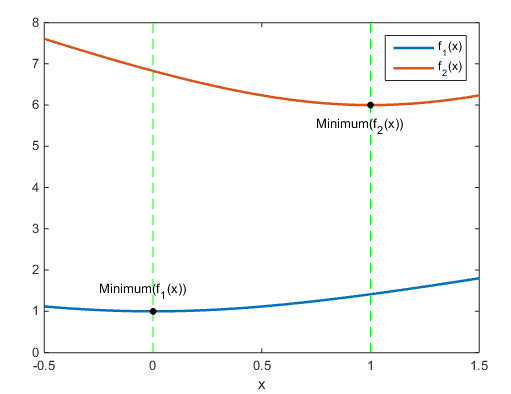
\includegraphics[width=7cm]{Thesis/LiteratureReview/VisualExTwoObj.png} }}%
    \qquad
    \subfloat[Tradeoff region due to weighted optimization.]{{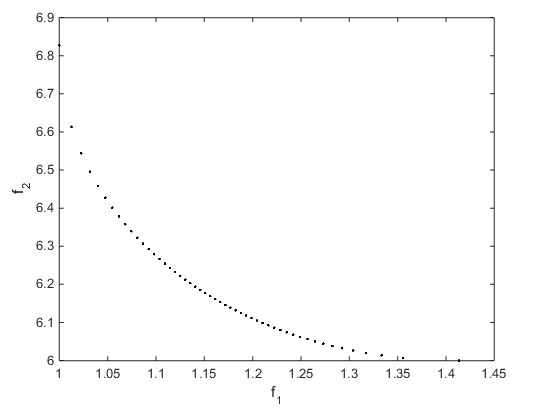
\includegraphics[width=7cm]{Thesis/LiteratureReview/VisualExTradeoff.png} }}%
    \caption{Example of a weighted Pareto Frontier.}%
    \label{visualex}
\end{figure}

By using multi-objective optimization, the Pareto Frontier shows the optimums given that one function is more important than another over this tradeoff region. Figure \ref{visualex}(b) shows the resulting tradeoff between the two objectives.


\par
Korhonen et al. \cite{MultOptCS} point out that there are two main methods when approaching a multiobjective optimization problem. These are the weighting method and the constraint method. In these two methods, the decision maker can control the solution process with their preferences.\par
\subsection{Weighting Method}
The weighting method involves solving the following multiobjective optimization problem,
\begin{equation}
\begin{aligned}
    & minimize \sum^k_{i=1} w_if_i(\mathbf{x})\\
    & subject \ to \ \mathbf{x}\in S,
\end{aligned}
\label{eq:weightEq}
\end{equation}
where $w_i\geq 0 \ \ \forall i = 1,\dots,k$ and each objective is normalized so that magnitudes are not a factor in the solutions. The solution to Eq. \ref{eq:weightEq} is weakly Pareto optimal, meaning that the solution is not necessarily unique. The solution is Pareto optimal if for all $i = 1,\dots,k$, $w_i>0$ or if the solution is unique \cite{MultOptCS}. The weighting method can be used as a decision tool to generate different Pareto optimal solutions for the decision maker to choose from. The main requirement for the use of a weighting method is a convex problem. The optimal solutions of some nonconvex problems can sometimes be found no matter the weights, but cannot be proven and does not always behave like the convex solution method \cite{MultOptCS}.\par
\subsection{$\epsilon$-Constraint Method}
The second method is the $\epsilon$-constraint method where one of the objective functions is selected to be optimized and the rest are used as constraints in the optimization problem. The form of this problem can be seen in Eq. \ref{eq:constraintEq}.
\begin{equation}
    \begin{aligned}
    \text{minimize} \ & f_i(\mathbf{x})\\
    \text{subject to} \ & f_j(\mathbf{x})\leq \epsilon_j \ \forall j = 1,\dots,k, \ j\neq l,\\
    & \mathbf{x}\in S.
    \end{aligned}
    \label{eq:constraintEq}
\end{equation}
\section{Aircraft Assignment Problem}
The aircraft assignment problem is an application of the assignment problem to target locations from a starting point. The assignment problem can consist of one aircraft and multiple locations, a one-to-one matching of aircraft to target locations, or multiple aircraft to a greater number of locations. An assignment problem is a combina (REFERENCE BOOK).\par
A mixed-integer linear program (MILP) is generally the designation of assignment problems, given that the constraints and objective function are linear and that an assignment is either fulfilled or not. In their paper on the UAV routing assingment problem, Shetty et al. \cite{Shetty} use a mixed integer linear program, where the main constraints are service level and weaponry constraints. The formulation serves as a traveling salesman problem (TSP), where the objective is to minimize cost, but all locations must be visited in the model. There is no upper-level constraint for ability to travel or service for any amount of time.\par
In contrast, Alighanbari et al. \cite{Alighanbari}, Schumacher et al. \cite{Schumacher}, and Taylor et al. \cite{Taylor}, use constrained optimization based on range, timing, or fuel ratios. The advantage of this is that it can mirror real-world scenarios such as UAV waypoints \cite{Alighanbari} or flight mapping for commercial airliners \cite{Taylor}. Though Taylor et al. \cite{Taylor} used the TSP formulation in their model, the idea of using fuel as a constraint accounts for all possible maneuvers in an aircraft.\par
Vitte \cite{OptimizeBreguet} discusses the continuous coverage of a target area using a time on station designation and assuming a constant idle time. This allowed for a maximization of time on station for a certain number of aircraft while meeting the constraints for turn-around time and outbound time for any particular aircraft. The combination of this idea while allowing for multiple target locations in an imperfect matching scheme will allow for a decision maker to maximize the priority of targets with limited resources.


\section{Conclusion}
Though the cited sources are a subset of how the Br\'eguet equations are used, the equations are shown to be a reliable way to define the range and endurance of an aircraft, given certain parameters. Additionally, the similarities between the range and endurance equation can be used to define a tradeoff region for multiobjective optimization of range and loiter time. The next chapter will define a methodology of how these equations will be formulated to allow for a tradeoff region and how each parameter is extracted from aircraft profiles.